\documentclass[12pt]{article}
\usepackage[english]{babel}
\usepackage{amsmath,amsthm}
\usepackage{graphicx}
\usepackage{amsfonts}
\usepackage{indentfirst}
\usepackage{lscape}
\usepackage[top=2.5cm,bottom=2.5cm,right=2.5cm,left=2.5cm]{geometry}
\usepackage{titlesec}
\usepackage{subfigure}
\usepackage{caption}

\setcounter{secnumdepth}{5}

% ----------------------------------------------------------------
\begin{document}
\section{ SIFT(scale-invariant feature transform)}
SIFT  is an algorithm used in sector of computer vision for detection and identification of similar elements between different numeric images.
The principal method proposed by the author David Lowe is to calculate the SIFT descriptors on images studied. These descriptors are numeric information which derived of local analysis of the image and they characterize the visual content of this image so that this one is independent of the scale, the framing, the angle of observation and the luminosity.
\subsection{Stages of the SIFT algorithm}
The first stage is to detect key-points on the image. Each key-point is characterize by coordonates  x,y on the image and a scale factor $\sigma$. After that it's necessary to ameliorate the precision of the key-point localisation.
\begin{itemize}
\item Scale-space extrema detection\\
The gradient scale factor is calculated for smooth the original image. This operation allow to delete details which radius are inferior at $\sigma$.
\begin{equation}
L(x,y,\sigma)=G(x,y,\sigma)*I(x,y)
\end{equation}

\begin{figure}[h]
    \center
    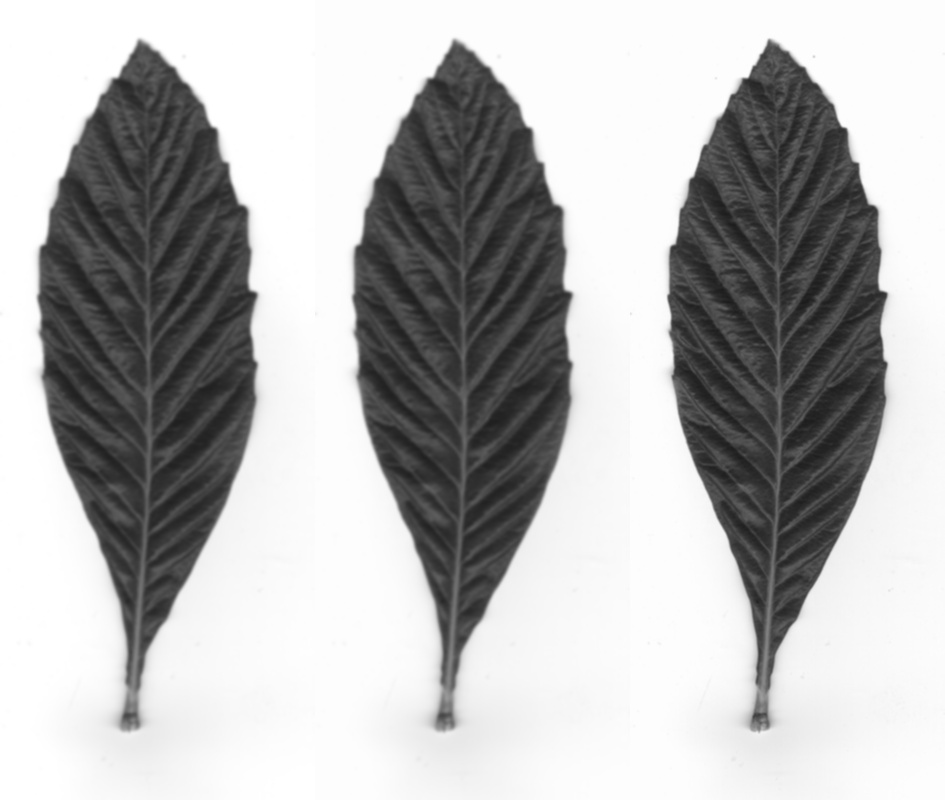
\includegraphics[scale=0.3]{blur.jpg}
    \caption{Illustration of scale factor gradient (octave 7x7;$\sigma_0$ =0; $\sigma_1$ =1.6; $\sigma_2$ =0.4) }\label{figure:Illustration of the scale factor gradient}
\end{figure}
After that, the key-points which have dimension approximately equal to $\sigma$ are detected by using the Difference of Gaussian(DoG) given by the following equation.
\begin{equation}
D(x,y,\sigma)=L(x,y,k\sigma)-L(x,y,k\sigma)
\end{equation}
Where k is the fixed parameter of the algorithm and depend to the fineness of the scale desired.
\begin{figure}[h]
    \center
    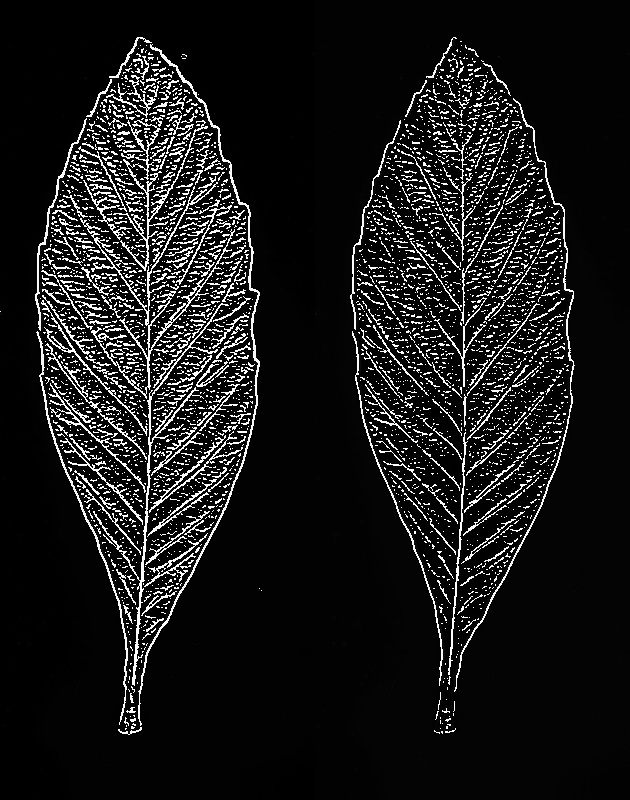
\includegraphics[scale=0.3]{DoG.jpg}
    \caption{Illustration of the DoG}\label{figure:Illustration of the DoG}
\end{figure}


\end{itemize}

\begin{itemize}
	
	\item Orientation assignment\\
	 On the base of local image gradient detections each key-point detected is assigned to one or many orientations. 

  With the symmetric finite difference, the gradient and the amplitude are calculated for each position around the key-point.
The calculation of these two factors is given by the following relations:
$$m(x,y)=\sqrt{(L(x+1,y)-L(x-1,y))^2+(L(x,y+1)-L(x,y-1))^2}$$
$$\theta(x,y)=atan2(L(x,y+1)-L(x,y-1),L(x+1,y)-L(x-1,y))$$
A histogram with 36 intervals is realized on the vicinity and each interval covering an angle of 10 degrees.

 The peaks in this histogram correspond to the dominant orientations. All dominant orientations allow to have at least 80\% of the maximum value are taking in consideration and other additional key-points are detected. These new key-points detected are only different by the principal orientation.

	\item key-point descriptor \\
An area of 16x16 pixels is taken around the key-point; subdivide in 4x4 zones of 4x4 pixels each one. A histogram including 8 intervals is calculated on each zone. 

After that, the 16 histograms with 8 intervals each one, are concatenated and normalized. In object to reduce the sensibility of the descriptor to the changes of the luminosity, the values are fixed to 0.2 and the histogram is calculated again for finally give the descriptor of the key-point of 128 dimension.
\end{itemize}

\section{ SIFT test and results}

In our project we used the SIFT  of  Opencv library in python. This function allow to detect key-points  on images and compute descriptors for each one.   
The script is adapted to our program in order to caculate  descriptors in whole database of images.
Before integreting the script in the process flow, test steps were done in order to verify if the results obtained with the program are satisfied.

Tests consist to apply the sift on image according to different configurations to notice the invariance of the function to the configurations.
In a first phase, the tests were done on a basic image design on paint. 
Here we have the illustration images  of the results

\begin{figure}[!h]
\centering     %%% not \center
\subfigure[Key-points detected ]{
\includegraphics[width=70mm]{test1.jpg}}
\subfigure[Key-points detected after luminosity change]{
\includegraphics[width=70mm]{lum1.jpg}}
\caption{Illustration 1}
\end{figure}

%\begin{figure}[!h]
   % \center
   % 
\includegraphics[scale=0.2]{scal1.jpg}
  %  \caption{Key-points detected after scale change}
   % \label{figure:Illustration }
  % \end{figure}
   

\begin{figure}[!h]
    \center
    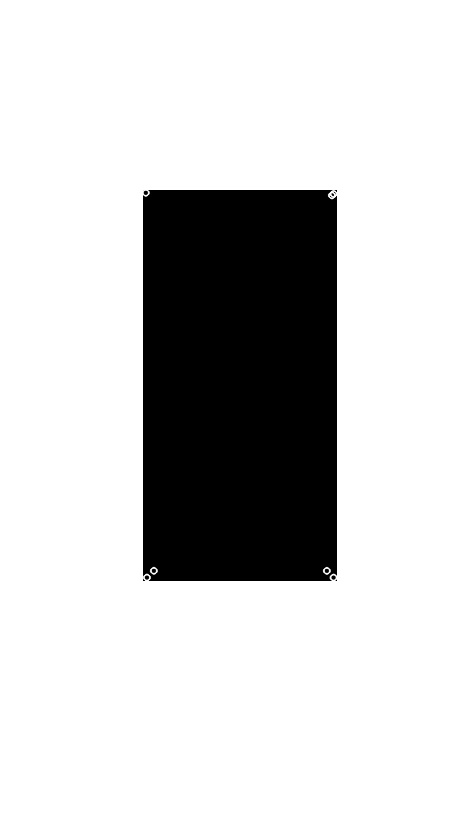
\includegraphics[scale=0.3]{rot1.jpg}
    \caption{Key-points detected after rotation}
    \label{figure:Illustration }
\end{figure}
\clearpage

After that, the test was also done on three images of the database. Three  images which look alike are taken in the database and key-points are calculated on each one. 
These images are matched two by two with the key-points in order to find similarity between images.

\begin{figure}[!h]
\centering     %%% not \center
\subfigure[Illustration 1 ]{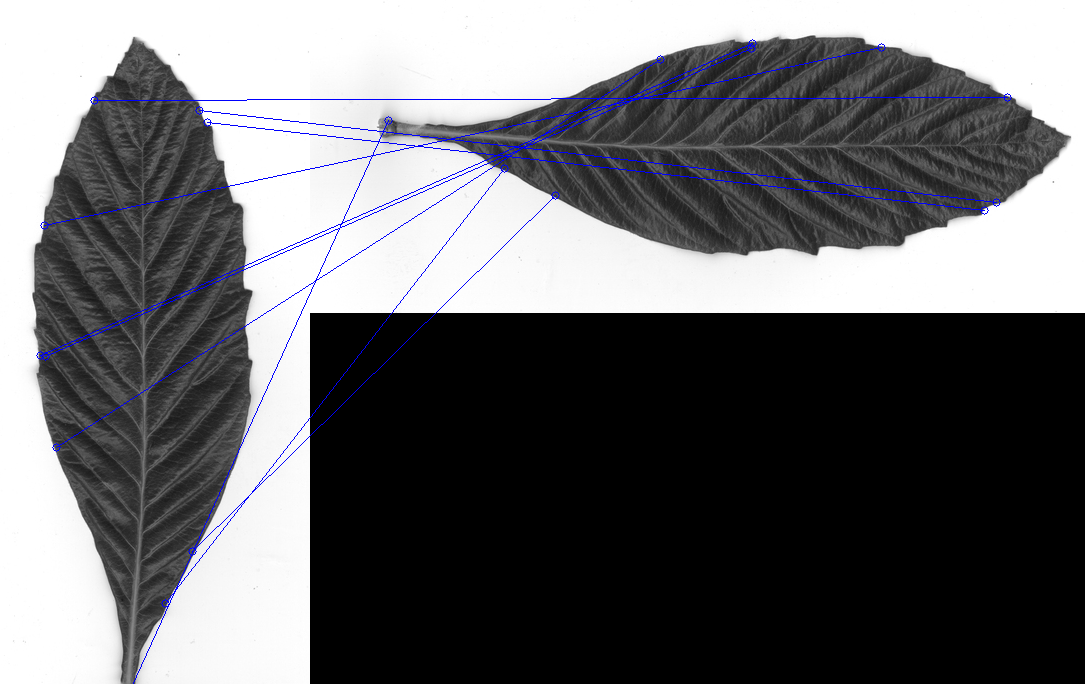
\includegraphics[width=50mm]{Capture2.png}}
\subfigure[Illustration 3]{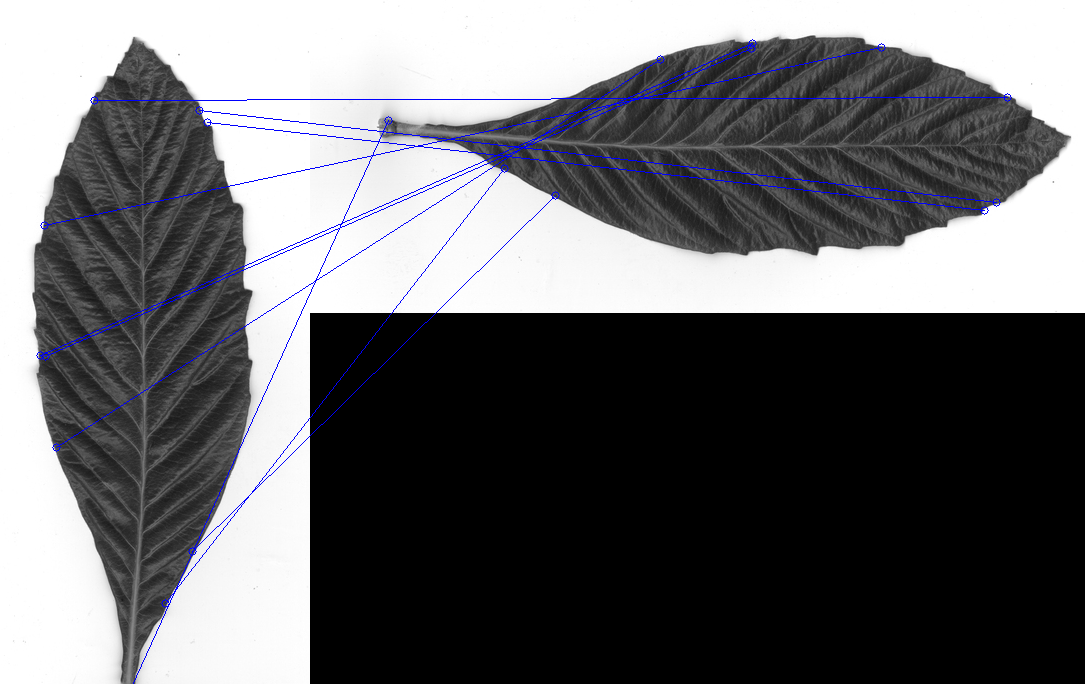
\includegraphics[width=50mm]{Capture1.png}}
\subfigure[Illustration 3]{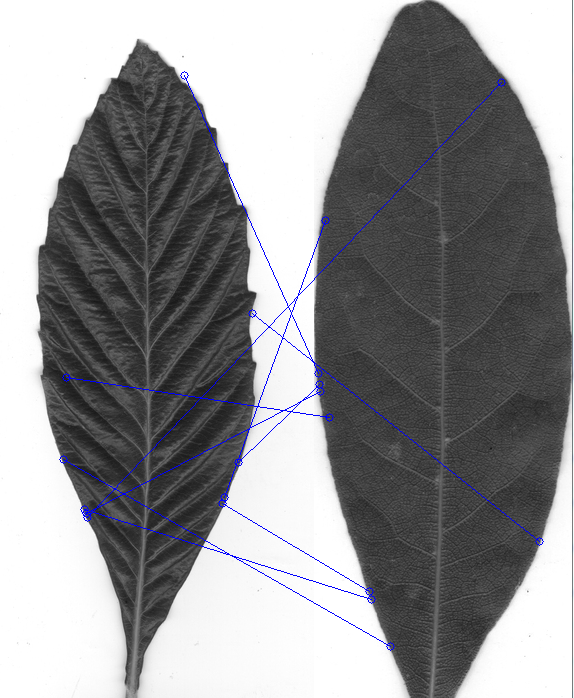
\includegraphics[width=50mm]{Capture.png}}

\end{figure}
 
 According to our relsults obtained through the images above, we concluded that the SIFT descriptor is satisfied and it can be used to compute all descriptors in whole the database. 
 
 \section{ Parallelism test}
 
This test consist to use multiple processors to make a computation faster. It will permit multiple tasks to proceed without waiting for each other.
The algorithme consist to decompose the complete task into independent subtasks and the data flow between them and distribut the subtasks over the processors.
In python we have different posibilities to do this. The test was done by using the module multiprocessing because it was the only avaible in our python version.
We can see on the following images the time computation before and after using the parallelism.

\begin{figure}[!h]
\centering     %%% not \center
\subfigure[Illustration with parallelism ]{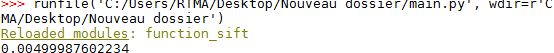
\includegraphics[width=100mm]{multi.png}}
\subfigure[Illustration without  parallelism]{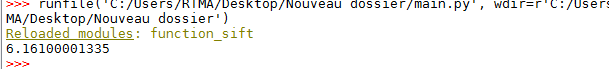
\includegraphics[width=100mm]{mult2.png}}
\end{figure}


 
 




% ----------------------------------------------------------------
\end{document}